
\documentclass[11pt,letterpaper,oneside]{article}
\usepackage[top=1in,left=1in,right=1in,bottom=1in]{geometry}
\usepackage{fancyvrb}
\usepackage{colortbl}
\usepackage{graphicx}
\usepackage{url}

\title{Arm ARUM with Dynamic Instrumentation}
\author{Dejun Qian, Deron Jensen, Amritha Nambiar, Sisinty Sasmita Patra\\Department of Computer Science\\Portland State University\\Portland, OR 97201\\dejun@pdx.edu}

\begin{document}
\maketitle

\begin{abstract}
Based on the initial implementation, we make ARUM, an Application Resource Usage Moniter for multi-core and multi-processor systems, capable of operating on application binaries, measuring the performance and resource usage at function level. Dyninst, a dynamic instrumentation library, is adopted to help communicate with application binaries at run time. This report presents how we improve ARUM. Experiment result shows that, with our effert in this project, ARUM is enhanced in forthfold, 1) provide the CPU usage not only at program level but also at function level. 2) give how many times each function is called. 3) provide the function call hierachy without reading the source code. 4) list the function implemented in the application.
\end{abstract}

% Include the motivation for your work, your approach, your goals, and a short summary of what you found/achieved/tested.
\section{Introduction}
\label{sec:introduction}
The performance data for both systems and applications plays a critical role in determining the causes of the poor performance of the applications, suggesting the ways to improve the applications, and providing baseline to comparing applications. Among a bunch of performance measuring tools, ARUM provides a unique all-in-one solution for collecting a variety of performance data with a single tool, while still keeping itself lightweight, easy-to-use. ARUM could do four measurements: process and thread level resource usage, architecture specific event counting, application level measurements, and measurements of the ambient environment. It does not need recompile, relink the application or change the source code of the application \cite{bib:knapp}.

However, in the initial implementation, only the first two measurement components have been done. In this project, we manage to implement the third one, which focus on extending ARUM to measure the performance of applications. Application level measurement give insight into the performance of an application. The measurement range from course-grained to fine-grained. For course-grained measurement, the overhead of the tool will be relatively lower, and will not affect the original behavier of the application. The cost of the least perturbation is the lack of detailed performance information. For example, if we measure a application in course-grained mode, then we only get the information about the execution of the application as a whole. The information about some certain pieces of code, like a function, is unknown in this mode. In contrast, for fine-grained measurement, we can get more detailed information about the execution of the application at the cost of higer overhead of the tool. The initial version\footnote{\texttt{\url{http://web.cecs.pdx.edu/~cs533acc/arum.git}}} we got to begin with have done the course-grained measurement. Our work in this project is mainly related to fine-grained measurement.

In order to avoid recompiling, relinking, and operate on application binary, we adopt Dyninst \cite{bib:dyninstweb} to communicate with the binary code of the application in testing. Dyninst is \cite{bib:anapi} a post-compiler program manipulation tool which provides a C++ class library for program instrumentation. Using this library, it's possible to instrumentate and modify application programs during execution. Using Dyninst, we successfully extend ARUM with four useful features: 1) provide the CPU usage at both program level and function level. 2) give the calling frequency of each function. 3) provide the function call hierachy. 4) list the functions implemented in the application.

The rest of the paper is orgnized as follows. Section \ref{sec:methodology} introduce our implementation to make ARUM provide fine-grained measurement of application binaries. Section \ref{sec:results} gives the experiment result of our implementation. Section \ref{sec:conclusion} conclude our work and give some thinking towards the future.

% Explain your design / languages, libraries, and tools used, experimental design.
\section{Methodology}
\label{sec:methodology}
This section presents what we have done and how we did it to make ARUM capable of fine-grained measurement, as well as let the code structure more clear and easy to mantain.

\subsection{Build and Make existing code}
On the first stage of our work, we tried to understand the initial version of ARUM code, reorganize the source code structure, add more help message and error message to make ARUM more robust and user-friendly. Basically, the following work is done,
\begin{enumerate}
\item Reorganized code into /src /test /tools with docs and makefiles.  Tests are now merged into test directories and linked to ARUM libraries.
\item Added Makefile and instructions for Hardware counter kernel module.
\item Added usable error messages and exceptions for unsupported hardware (IA32).
\item Added accurate "usage" message to output.
\item Added environment variable for HwCtr module configuration and '-r' flag to allow ARUM to run on unsupported hardware, or outside of the "make" area.
\end{enumerate}

\subsection{Dynamic Instrumentation}
\textbf{Dyninst}\newline
\indent Dyninst is a library developed at University of Maryland and University of Wisconsin Madison. It is a dynamic instrumentation tool which operates on application binary only, without re-compiling, re-linking or even re-executing. This library permits the insertion of code into an application that is either running or on disk. Basically, there are two ways to insert code into the application binary, namely, dynamic instrumentation and static instrumentation. Dynamic instrumentation inserts code into a running application while static instrumentation inserts code into an executable file or library \cite{bib:dyninstmanual}.

\begin{figure}
\begin{center}
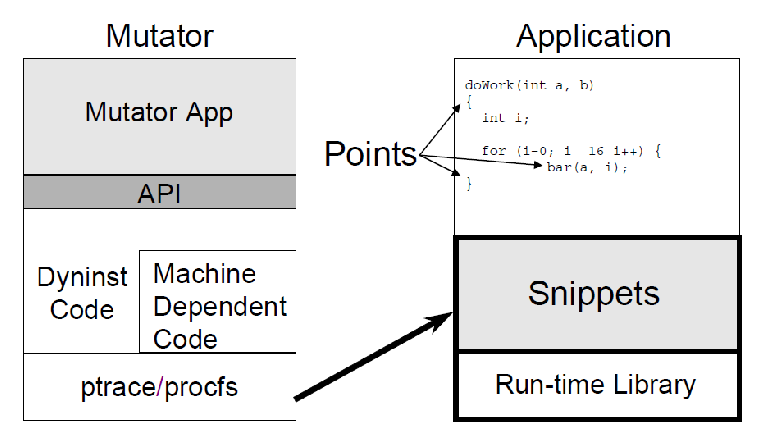
\includegraphics[width=0.6\textwidth]{dyninst.eps}
\caption{Structure of Dyninst}
\label{fig:dyninst}
\end{center}
\end{figure}

How Dyninst works is illustrated in Figure \ref{fig:dyninst}\footnote{\texttt{from Bryan's paper \cite{bib:anapi}}}. A \emph{point} is a location in a program where instrumentation can be inserted. A \emph{snippet} is a bit of binary code to be inserted into a point. The snippet is first prepared and dynamically compiled in the mutator's process space. The mutator then copies the snippet and other necessary libraries into mutatee's process space by using Linux's ptrace service. It also slightly revises the code of the \emph{point} in the mutatee to call the snippet. This way, Dyninst can insert the code into and control the execution of the mutatee.

\noindent \newline\textbf{Instrument Using Dyninst}\newline
\indent Figure \ref{fig:workflow} gives a general idea about how Dyninst works with ARUM. To do instrumentation with Dyninst, we should first integrate the Dyninst library into ARUM, then use the APIs provided by Dyninst to create a image of the application binary, prepare and insert the snippets into the specified points in the application image, then save the modified image as the new modified application binary, run the new executable binary. At this point, we should have two program running, one is the ARUM program, which is the mutator, the other is the modified application binary, which is the mutatee. The snippet in the mutatee is responsible to collect the performance data of the mutatee and send it to ARUM. After getting the data from mutatee, ARUM precess them and generate the performance report of the mutatee.

\begin{figure}
\begin{center}
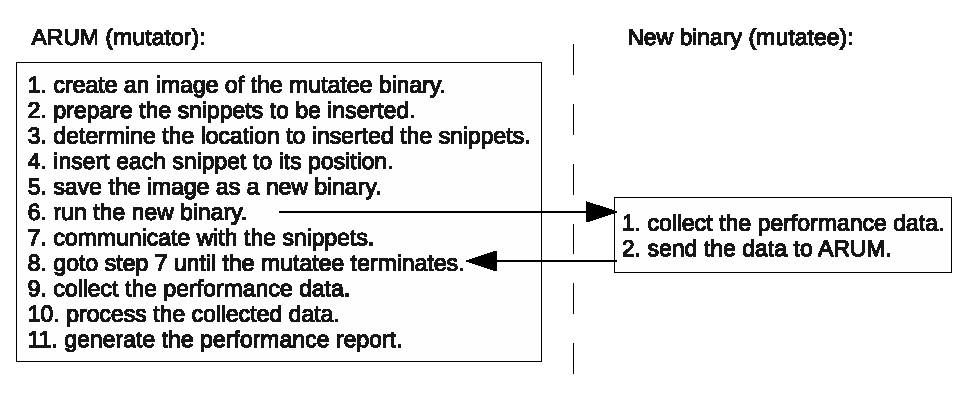
\includegraphics[width=0.9\textwidth]{workflow.eps}
\caption{Workflow of ARUM}
\label{fig:workflow}
\end{center}
\end{figure}

How the snippets are designed and where should they be inserted is the most important two question when we design our approach. The answer to these two questions depend on what performance we try to moniter. In this project, we try to profile the application program, which means we want to get how long does each function call take and how many time does each fuction is invoked. With this purpose, we designed four snippets: timestamp, isrecursive, preprocess and sendresult. The first one is used to get the timestamp of curcurrent point of execution, we use times() function in Linux. With this function, we can get the user time, system time and watch time. We insert this snippet into the beginning and the end of each function. Preprocess snippet simply collect the time at the beginning and at the end, while sendresult snippet send the result to ARUM.

There is one 

By passing the application name to ARUM as an argument, ARUM can open the binary file, parse the ELF format, and create an image to represent the application executable binary. The code used to achieve this goal is shown bellow,
\begin{Verbatim}[frame=single]
handle = bpatch.openBinary(app_name);
image = handle->getImage();
\end{Verbatim}

To instrument the application, we must first decide what data want to be collected, then proper snippet should be designed carefully. This is the most chanllege and most important task. Dyninst provide a bunch of APIs to help the user to create the snippets. These APIs can support bisic arithmetic computations, general assignment, conditional assignment, loop, function call and etc.. Using these APIs to write snippet code is very different from writing code using high level language. The code shown bellow gives an example of snippet which implementing increasement functionality.
\begin{Verbatim}[frame=single]
count = handle->malloc(*(image->findType(``int'')));
countPlusOne = new BPatch_arithExpr(BPatch_plus, *count, BPatch_constExpr(1));
incCount = new BPatch_arithExpr(BPatch_assign, *count, *countPlusOne);
\end{Verbatim}

Having the snippet ready, we can use Dyninst to locate the position where we want to insert the snippet, and then insert our snippet there. After that, when the application runs, our snippet code will get executing at certain position of the application. Of course, before we call Dyninst APIs, we should give the information about which function we are working on. The sample code to insert the above snippet is shown bellow,
\begin{Verbatim}[frame=single]
entry_point = function->findPoint(BPatch_entry);
handle->insertSnippet(*incCount,*entry_point);
\end{Verbatim}

Up to now, we can only instrument the manually specified function. With the code shown bellow, we can get the function list in the application and apply the above method to each of the function in the list. This way, we can automatically instrument all the functions implemented in the mutatee.
\begin{Verbatim}[frame=single]
image->findFunction(``main'', mainfuncs);
module = mainfuncs[0]->getModule();
return module->getProcedures();
\end{Verbatim}

For the purpose of profiling the application in binary image, we have collected enough information for further process. Based on these information, we can
\begin{enumerate}
\item recover the executing sequence of each function, when it begins and when it finishs.
\item give how many time does each function run
\item give how long does each function instance take to run in user time, system time and watch time.
\item give the average time each function takes to run.
\item give the calling hierarchy of the functions in the application.
\end{enumerate}
These task can be done by project 2. Using a good visualization technique will help Arum to present these information in a user friendly way.

After downloading Dyninst\footnote{\texttt{\url{http://www.dyninst.org/sites/default/files/downloads/dyninst/dyninst_linux_amd64_7.0.tar.gz}}}, we need install libiberty if working on linux server at PSU. The appropriate environment variables should be set according to where you put the libraries. Our settings are shown bellow,

\begin{Verbatim}[frame=single]
export LD_LIBRARY_PATH=../bprobe/lib:$LD_LIBRARY_PATH
export LD_PRELOAD=$(pwd)/../bprobe/lib/libdyninstAPI_RT.so
export DYNINSTAPI_RT_LIB=$(pwd)/../bprobe/lib/libdyninstAPI_RT.so
export DYNINST_LIBC=$(pwd)/../bprobe/lib/libc-2.13.so
\end{Verbatim}

Having set the required environment, we design our dynamic instrumentation library libbinpro.so based on Dyninst. The command used to build our library is shown bellow,

\begin{Verbatim}[frame=single]
$(CC) $(CXXFLAGS) -shared -fPIC -Wl,-rpath=./lib binpro.o -L./lib -ldyninstAPI
      -ldwarf -linstructionAPI -lsymtabAPI -lcommon -lparseAPI
      -o ./lib/libbinpro.so
\end{Verbatim}

When successfully get the library libbinpro.so, we integrate this library with ARUM, and make ARUM capable of dynamic instrumenation. Because the library libcommcon.so have some unresolved function provided by libiberty.a, we need the command bellow to build ARUM,

\begin{Verbatim}[frame=single]
$(CXX) $(CXXFLAGS)-rdynamic -Wl,-rpath=../bprobe/lib $(ARCHIVE) -L../bprobe/lib
      -lbinpro -Wl,--whole-archive -liberty -Wl,--no-whole-archive
      -o $(EXE)
\end{Verbatim}


We use Dyninst to inject binary code into the application binary. We extend Arum in the following way:
\begin{enumerate}
\item Build Dyninst library and integrate it into Arum.
\item List all the functions in the application along with the begining and end address of the code of each function.
\item Write the code to be injected into the application binary. The code will get the user time, system time and watch time at the executing time.
\item Inject the code into the begining and end of each function in the application.
\item Designed a machenism to pass the collected information from the application to Arum.
\item Generate the profiling report.
\item Designed a program to consume both measurable user time and measurable system time for testing purpose.
\end{enumerate}

stack

\textbf{Testing}
\begin{enumerate}
\item Test ARUM command line options and existing functionality.
\item Test a function call.
\item Test a loop and recursive function call.
\end{enumerate}

For ARUM, we looked at gprof style of output and Dyninst for dynamic instrumentation.  First, we needed to organize the ARUM code into a solid make and build exisiting tests with the ARUM code (not copies of the code).   Additionally we needed test cases for the new functionality, and a driver to test the programs.

The task of profile the application in binary mode is not trivial. We encountered the following challenges:
\begin{enumerate}
\item ARUM source code was duplicated and in several dispserse directories.  
\item Did not compile on IA32 (and other architectures).
\item HwCtr Module does not work as described in example (Don't know where the code is?)
\item Dyninst has several requirements to install and get working.
\item Can't use createProcess function. As a result, we can't inject the code into a running process. This problem is solved by rewriting the application binary before running the application.
\item Create customized structure when invoking times function to get the timestamps.
\item How to communicate with Arum as easy as possible.
\item Handle recursive function calls.
\end{enumerate}

To test this feature, we designed a test program which use noticable use time and system time. The functions implemented in the test program is listed in Fig \ref{fig:fake} - Fig \ref{fig:main}. In fig \ref{fig:fake}, we implement a function which will never be called in the program. Fig \ref{fig:foo} implement a funtion which spend competable time in user mode and kernel mode. Fig \ref{fig:recursive} is used to test recurseve functions. Fig \ref{fig:main} is the main function of the program.

\begin{table}[th]
\caption{Functions implemented in hello}
\centering
\begin{tabular}{rl}
\hline
Function & Description \\
\hline
fake & functioin never called \\
foo  & basic function \\
recursive & function call itself recursively \\
main & main function \\
\hline
\end{tabular}
\label{table:mutatee}
\end{table}

% This should NOT be raw data or code listings.  Instead you should present the key results from your work.  Be guided by the papers you have read this quarter - in cases where it is necessary for understanding, a small section of code might be listed, separate from the text, but more commonly an algorithm might be shown.  Results are not long tables of data, rather, one or two graphs, or tables with key rows or columns highlighted or italicized.
\section{Results}
\label{sec:results}
The result for the experiment is shown in fig \ref{fig:orig} - fig \ref{fig:trace}. Fig \ref{fig:orig} shows the result of the original version of Arum we get from the project assignment. From this point, we only get the user time and system time of the whole program. There is no value to have this information to improve the performance of the program, as it didn't give us where does the program need to be improved. Fig \ref{fig:list} is the result of the function list of the program output by the new version of Arum which is extended by this project. The is the first step of our implementation. This list can give us a general idea about the size of the program. The more functions the program has, the more complex the program is. Fig \ref{fig:trace} shows the execution trace of the program. The information includes the beginning time and end time of each function of both user time and system time as well as watch time. With these information, we can figure out which function is called more and need more attension.
\begin{figure}
\begin{center}
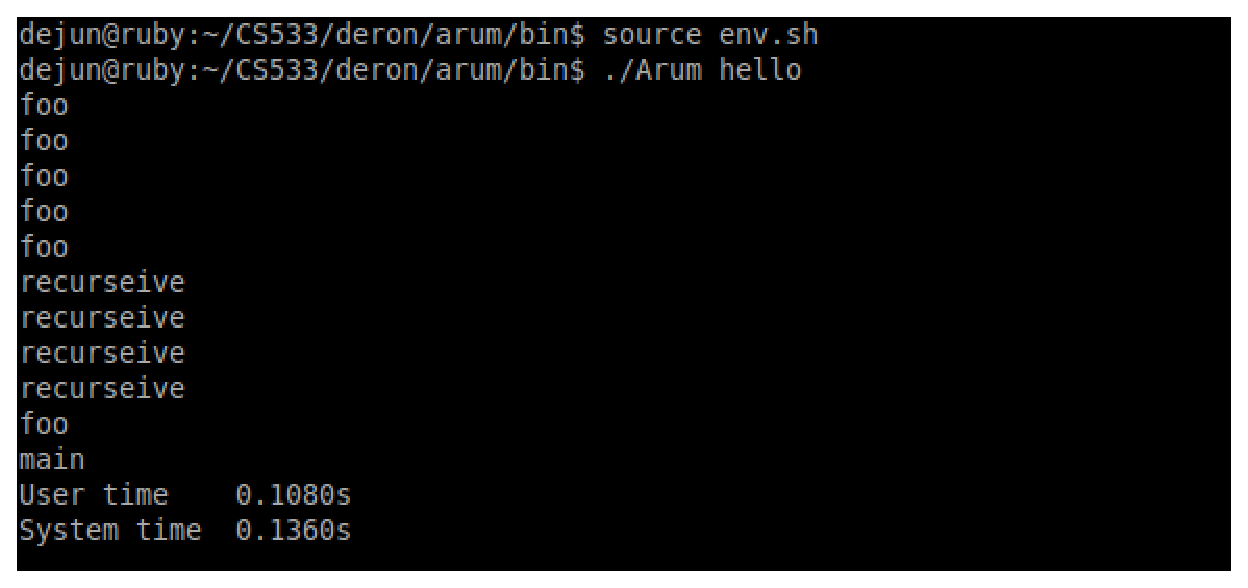
\includegraphics[width=6in]{orig.eps}
\caption{output from the original}
\label{fig:orig}
\end{center}
\end{figure}
\begin{figure}
\begin{center}
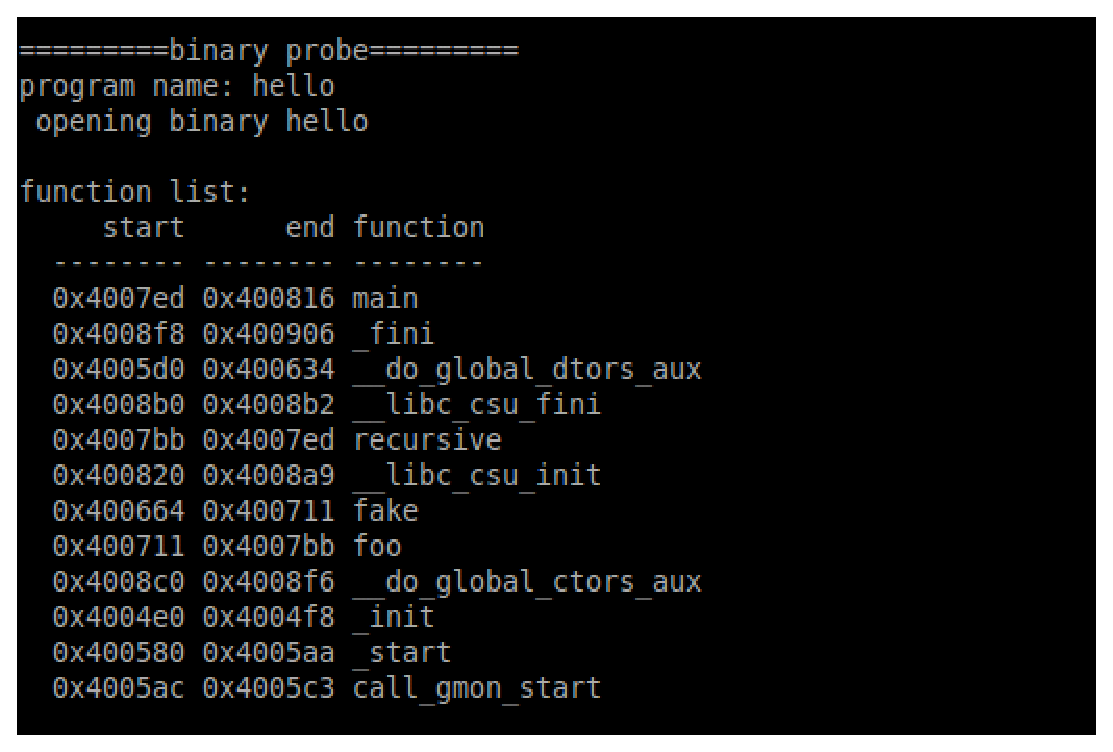
\includegraphics[width=6in]{list.eps}
\caption{function list}
\label{fig:list}
\end{center}
\end{figure}
\begin{figure}
\begin{center}
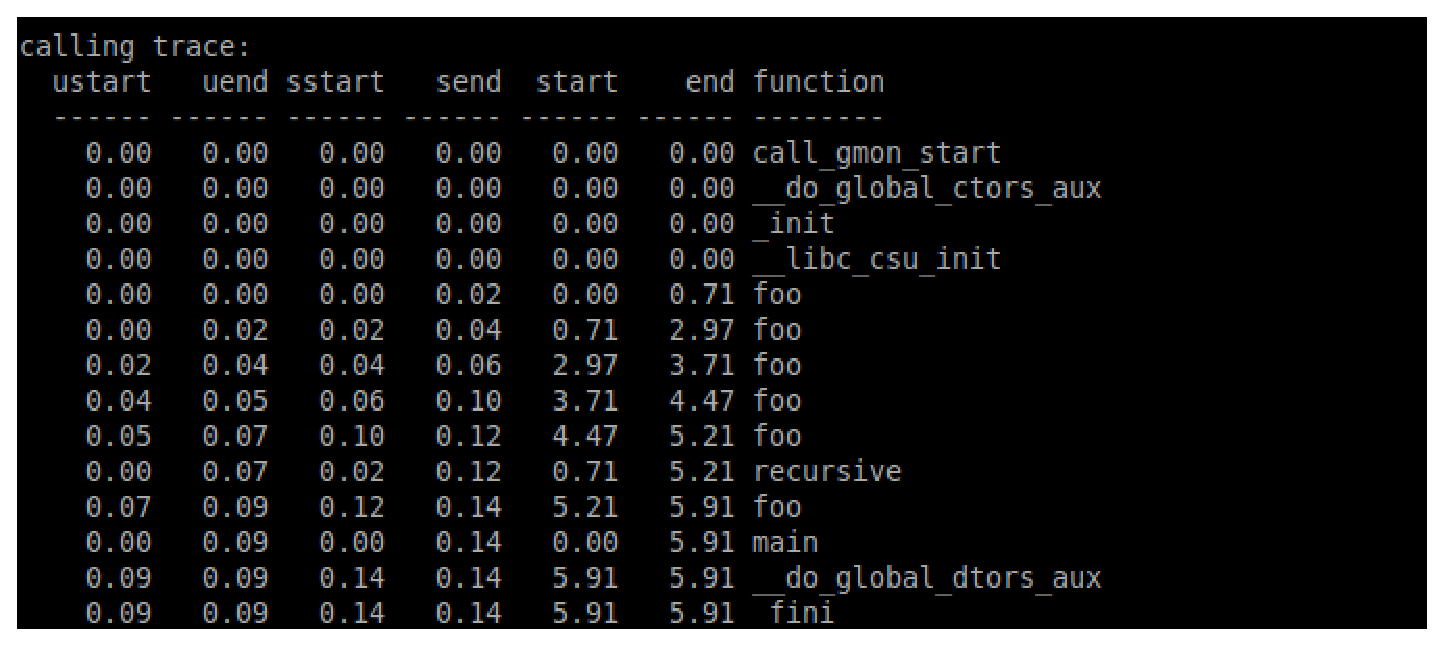
\includegraphics[width=6in]{trace.eps}
\caption{execution trace}
\label{fig:trace}
\end{center}
\end{figure}

% Based on what you have so far, what can you conclude?  What cool ideas did you think up but not have time to implement so far?
\section{Conclusions and Future Work}
\label{sec:conclusion}
There is still a great deal of opportunity to improve ARUM.   One of the future goals should be to allow ARUM to run on other hardware.  The kernel module currently only supports a single architecture (Intel-15-6).  Adding the Dyninst modules to the build is extremely difficult.  Dyninst requires much work to install on various architectures and platforms.   Currently the Dyninst is compiled and commited with the project.  It should be added as a separate module outside of the project.  Additionally the ARUM build should link with the location of the Dyninst.
\newline
The current instrumentation works, but needs to do some formatting of the output.  The data is available, but there may be other ways to present the information to the user of the program.
\newline
There are several tests that still need to be implemented to fully test all the functionality:
\begin{enumerate}
\item Planning to do tests for the command line option flags which give information of other metrics as well. 
\item Planning to come up with a test program that can be used as benchmark application for testing Arum functionalities with the ability to test features of Arum that include command line options, profiling for a single function, number of times the function is called and update test scripts once the	testing is automated.
\item Plan to use Arum as well as a widely-used profiling tool like gprof on the benchmark test application to compare and measure the efficiency,	overheads or improvements that can be done on Arum. 
\end{enumerate}

% Follow a standard ACM format for your references.  You have examples in the papers you have read.
\bibliographystyle{acm}
\bibliography{reference}

%\begin{thebibliography}{9}
%\bibitem{bib:dyninst}
%\emph{http://www.dyninst.org}
%\bibitem{buck}
%Buck, B., Hollingsworth, J. \emph{An API for Runtime Code Patching}. Computer Science Department: University of Maryland. 
%\bibitem{bib:knapp}
%Knapp, R. L., Pase, D. M., Karavanic, K. L. \emph{ARUM: Application Resource Usage Monitor}.  Computer Science Department:  Portland State University.
%\end{thebibliography}

\end{document}
